\chapter{Lab 3: ARP, IP, and ICMP}\label{Lab3}

\section{Objective}
%List objectives of the lab

\noindent In this lab, we will investigate the Address Resolution Protocol~(ARP), the IP~(Internet Protocol), and Internet Control Message Protocol~(ICMP). The first part of this lab is mainly about the ARP protocol. We will study the operation of the protocol based on the fields that it sets in the Ethernet frame containing the ARP message.  The second part of the lab focuses on analyzing IP frames, by observing and interpreting the fields in the IP frame. The last part of this lab focuses on the format and content of the ICMP messages.

\section{Introduction}
%Introduce the theory behind what we are going to be doing in the lab
\subsection{Address Resolution Protocol~(ARP)}
\par ARP is the standard method for finding a host's hardware address when only its network layer address is known.  It can be used to resolve many different network-layer protocol addresses to hardware addresses. Due to the overwhelming prevalence of IPv4 and Ethernet, ARP is primarily used to translate IP addresses to Ethernet MAC addresses. ARP is used in the following four cases when two hosts communicate:
\begin{enumerate}

\item When two hosts are on the same network and one desires to send a packet to the other.

\item When two hosts are on different networks and must use a gateway/router to reach the other host.

\item When a router needs to forward a packet for one host through another router.

\item When a router needs to forward a packet from one host to the destination host on the same network.
\end{enumerate}

\noindent The first case is used when two hosts are on the same physical network (that is, they can directly communicate without going through a router). The last three cases are the most used over the Internet as two computers on the Internet are typically separated by several hops.

\subsection{Internet Protocol~(IP)}
\par Above the link layer, there is the network layer, which is responsible for relay the date between the transport layer and the link layer. The network protocol in network layer is called the Internet Protocol, or more commonly, the IP Protocol. The IP protocol performs two basic functions, the addressing~(IP address) and the packet routing. Note that the internet layer is agnostic of application data structures as the transport layer, and it also does not distinguish between operation of the various transport layer protocols. Thus, IP protocol can carry data for a variety of different upper layer protocols by different protocol numbers, such as TCP, UDP and ICMP. \\

\noindent There are currently two versions of the IP protocol, IPv4 and IPv6. In this section we examine IPv4, which the most widespread version. With given trace files, we're going to learn about the details of IP frame. 

\subsection{Internet Control Message Protocol~(ICMP)}
\par The Internet Control Message Protocol~(ICMP) is one of the core protocols for network management in the Internet. It is mainly used by networked computers' operating systems to send error messages — indicating, for instance, that a requested service is not available or that a host or router could not be reached. It has been used in network trouble-shooting and analyzing applications such as \textit{ping} and \textit{traceroute}.\\

\noindent ICMP uses the basic support of IP as if it were a higher level protocol; however, ICMP is actually an integral part of IP, and must be implemented by every IP module. ICMP messages are sent in several situations: for example, when a datagram cannot reach its destination, when the gateway does not have the buffering capacity to forward a datagram, and when the gateway can direct the host to send traffic on a shorter route~[RFC792].\\

\noindent In this part of the lab, we use two network tools. One is \textit{ping}, which is used to test whether a particular host is reachable across an IP network, to self-test the network interface card of the computer, or to measure latency. The other one is \textit{traceroute}, used to determine the route taken by packets across an IP network.  We can understand the functions of ICMP by using these tools.

\section{Procedures}
%List procedures of the lab
\subsection{Exploring ARP functions}\label{Pro_ARQ}
\begin{itemize}
\item Download and open the trace named ``ethernet-trace-1''.

\item This trace basically emulates retrieving a long document.

\item The ARP protocol typically maintains a cache of IP-to-Ethernet address translation pairs on your computer.

\item Find the ARP request message and answer questions~(1)-(5) in section~\ref{Dis_ARP}.

\item Find the ARP reply that was sent in response to the ARP request and answer questions~(6)-(10) in section~\ref{Dis_ARP}.
\end{itemize}

\subsection{Analyzing IP frames}\label{Pro_IP}
\begin{itemize}
\item Using the same trace file as above.

\item Select any packet with the HTTP GET message in the trace and expand the IP header fields~(using the “+” expander or icon) to see the details. You can simply click on a packet to select it~(in the top panel). And the details of its structure~(in the middle panel) and the bytes that make up the packet~(in the bottom panel). Our interest is the IP header, and you may ignore the other higher and lower layer protocols. 

\item Select the the packet with HTTP GET message~(the No.10 packet) and answer questions~(1)-(2) in section~\ref{Dis_IP}.

\item Observe all the packets and answer questions~(3)-(4) in section~\ref{Dis_IP}.
\end{itemize}

\subsection{Exploring ICMP functions}\label{Pro_ICMP}
A. {\em Ping} The {\em ping} program in the source host sends a packet to the target IP address; if the target is alive, the {\em ping} program in the target host responds by sending a packet back to the source host. Both of these {\em ping} packets carry ICMP messages.\\

\noindent The following procedures describe how to capture the traces of ping messages.
\begin{itemize}
\item Start up the WireShark and begin packet capture.
 
\item Open a console, type the command \textit{ping www.engr.uvic.ca -c 10\footnote{The \textsl{ping} command here is different in Linux and Windows operating system. If you're working in Windows system, the command here should be \textsl{ping www.engr.uvic.ca -n 10}}} in the command line. The argument ``-c 10'' indicates that ten ping messages should be sent.

\item When the {\em ping} program terminates, stop the packet capture.

\end{itemize}

\noindent Download and open ``ping-trace-1'' in WireShark. Use the display filter to list the ICMP messages only, as shown in Figure~\ref{Lab3_fig_1} and answer questions~(1)-(4) in section~\ref{Dis_ICMP}.
\begin{figure}[hbt]
\centering
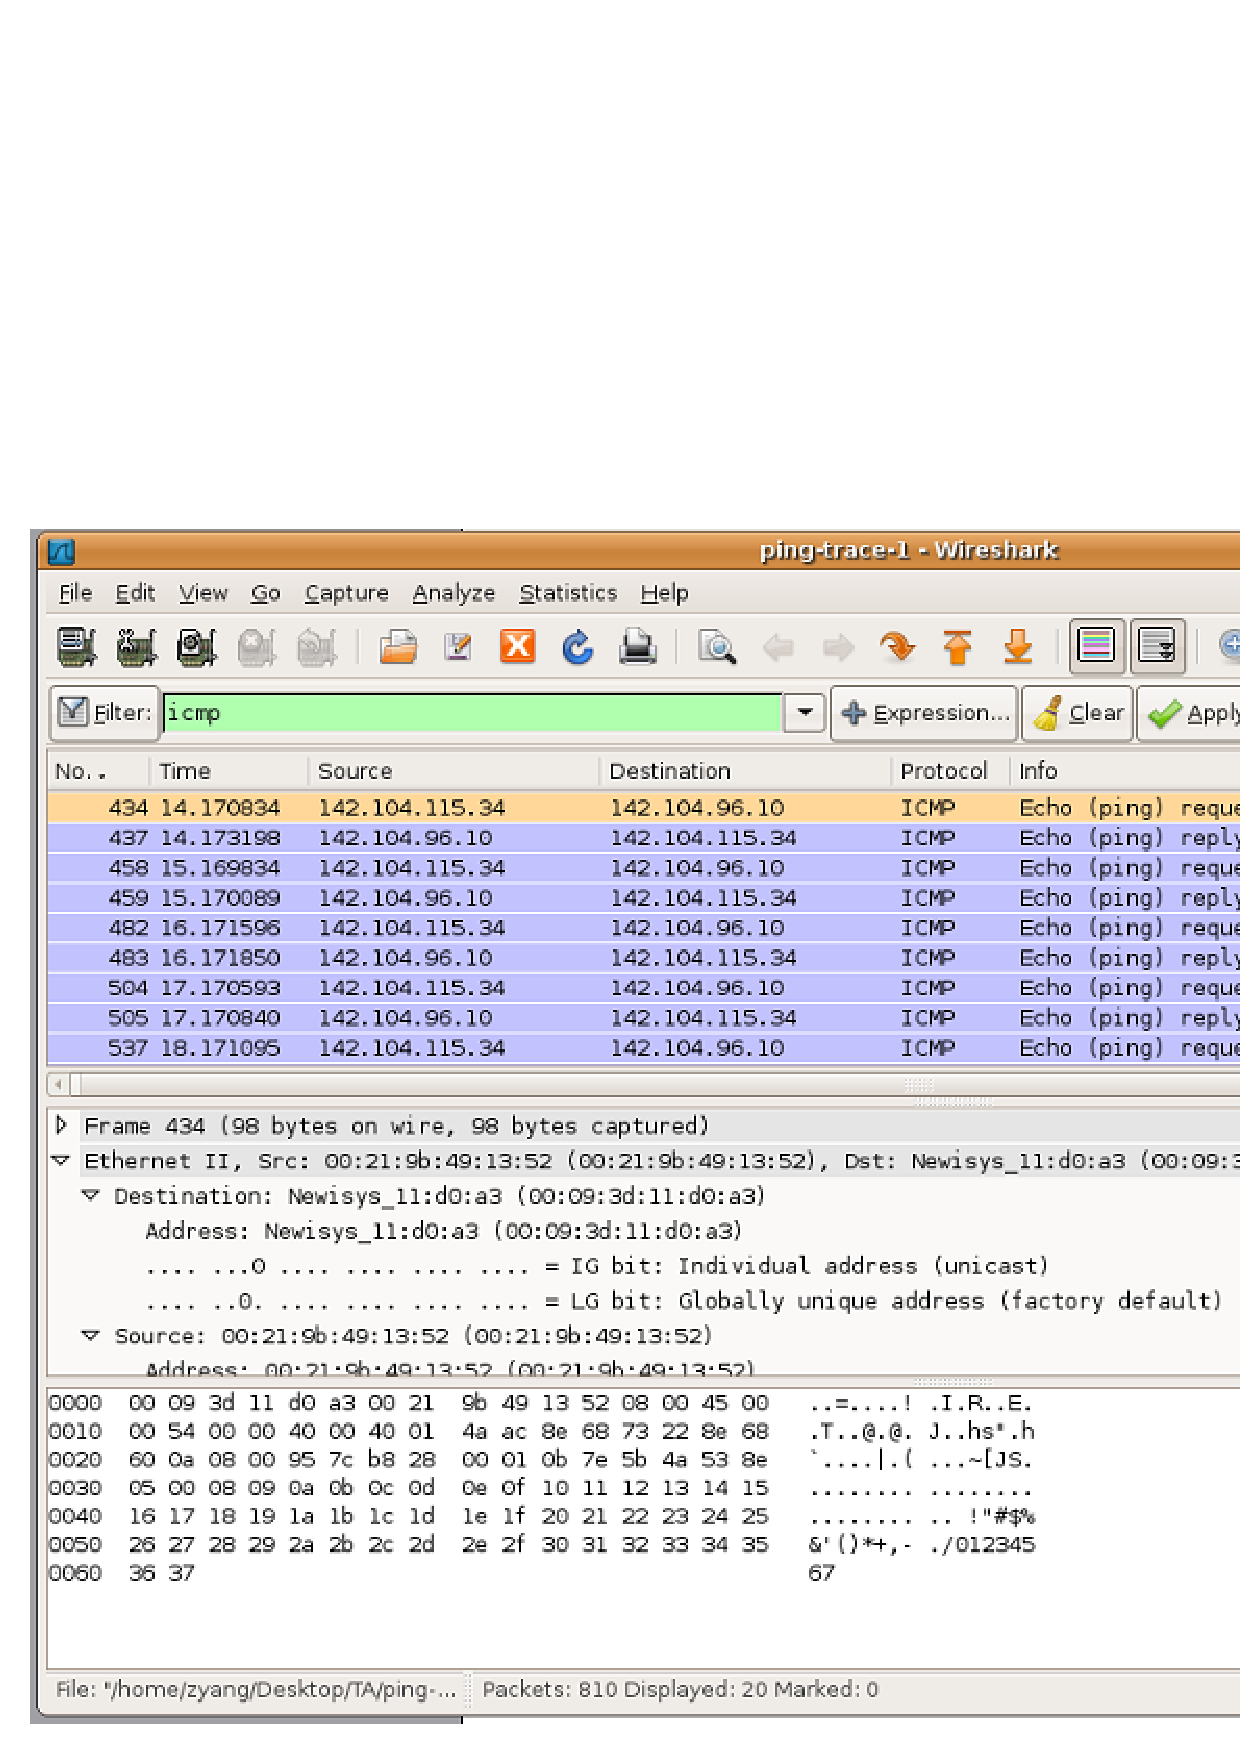
\includegraphics[width=5.5 in,angle=0]{Lab3_fig_1}
\caption{Capture of {\em ping} packet with ICMP display filter} \label{Lab3_fig_1}
\end{figure} \\

\noindent B. {\em Traceroute} The {\em traceroute} program is used to figure out the path a packet takes from the source to the destination. The following procedures describe how to capture the packets of traceroute messages.

\begin{itemize}
\item Start up the WireShark and begin packet capture.

\item Open a console, type the command \textit{traceroute www.engr.uvic.ca} in command line.

\item When the \textit{traceroute} program terminates, stop the packet capture.

\end{itemize}

\noindent Download and open ``tracert-trace-2'' in WireShark, and set the display filter as \textit{icmp}. Then answer the questions~(5)-(7) in section~\ref{Dis_ICMP} based on the trace.

\section{Discussion}

\subsection{Exploring ARP functions}\label{Dis_ARP}
\noindent  Answer the following questions based on the trace file ``ethernet-trace-1''.

\begin{enumerate}

\item What are the hexadecimal values for the source and destination addresses in the Ethernet frame containing the ARP request message?

\item Find the hexadecimal value for the two-byte Ethernet Frame type field. 

%\item What do the bit(s) whose value is $1$ mean within the flag field?

%   \item Discribe the content of the Ethernet frame (containing the ARP message). What are the values and meanings of these fileds?

\item  Where the ARP opcode~(operation code) field is located, i.e., how many bytes bits are there between of first bit of the opcode and the first bit of the ARP message?
%How many bytes from the very beginning of the Ethernet frame does the ARP opcode field begin?

\item What is the value of the opcode field within the ARP-payload part of the Ethernet frame, in which an ARP request is made?

\item Does the ARP message contain the IP address of the sender?
   
%\item Which field contains the MAC address of the host whose corresponding IP address is being queried, and what is it?

\item Where the ARP opcode field is located, i.e., how many bytes from the very beginning of the Ethernet frame does the ARP opcode field begin?

\item What is the value of the opcode field within the ARP-payload part of the Ethernet frame in which an ARP response is made?
      
\item What is the MAC address answered to the earlier ARP query?
      
\item What are the hexadecimal values for the source and destination addresses in the Ethernet frame containing the ARP reply message?
  
\item Why there is no ARP reply for the second ARP query~(packet No.6)?
\end{enumerate}

\subsection{Analyzing IP frames}\label{Dis_IP}
Answer following questions based on ``ethernet-trace-1''.
\begin{enumerate}

\item Sketch a figure of \textbf{the packet you selected} to show the position and size in bytes of the IP header fields, as well as the values in hexadecimal. Your figure can simply show the frame as a long, thin rectangle. 
	
\item What are the IP and MAC addresses of the source and destination?
	
\item How does the value of the Identification field change or stay the same for different packets? Is there any pattern if the value does change?	
	
\item How can you tell from looking at a packet that it has not been fragmented? 
\end{enumerate}

\subsection{Exploring ICMP functions}\label{Dis_ICMP}
Answer following question based on ``ping-trace-1'' and ``tracert-trace-2''.

\begin{enumerate}
\item What is the IP address of the source host~(client)? What is the IP address of the destination host~(server)?

\item  Can you get the average RTT (Round Trip Time)? What's that?

\item Examine one of the ping request packets. What are the ICMP type and code numbers? What other fields does this ICMP packet have? How many bytes are the checksum, sequence number and identifier fields?

\item Examine the corresponding ping reply packet. What are the ICMP type and code numbers? What other fields does this ICMP packet have? How many bytes are the checksum, sequence number and identifier fields?\\

\item What is the IP address of the source host~(client)? What is the IP address of the destination host~(server).

%\item Is there any difference between the request and reply packets from ``ping-trace-1'' and ``tracert-trace-2''? Why so?

\item Examine the ICMP error packet, which could be found in the
  packets from \textit{tracert-trace-2}. It has more fields than the
  ICMP echo packet. What are included in those fields? Find the TTL
  field, and explain what is it?

\item How many routers are between the source and the destination~(\textsl{www.engr.uvic.ca}), for the trace file? Please draw a figure to show the sequences of these routers, i.e, source --$>$ router\_\textsl{first} --$>$ ... --$>$ router\_\textsl{last} --$>$ destination?

\item Can you get the average RTT times between the source host and each router? What are they?

\end{enumerate}

